\documentclass[tikz,border=5pt]{standalone}
\usepackage{amsmath}

\definecolor{corba}{HTML}{365FB3}
\definecolor{mesura}{HTML}{B91C1C}
\definecolor{fons}{HTML}{F4F7FC}

\tikzset{
  panell/.style={draw=black!18, rounded corners=4pt, fill=fons, line width=.6pt},
  figura/.style={draw=corba, very thick, fill=corba!8},
  guia/.style={draw=black!45, densely dashed},
  etiqueta/.style={text=mesura, font=\small},
  titol/.style={font=\bfseries},
}

\begin{document}
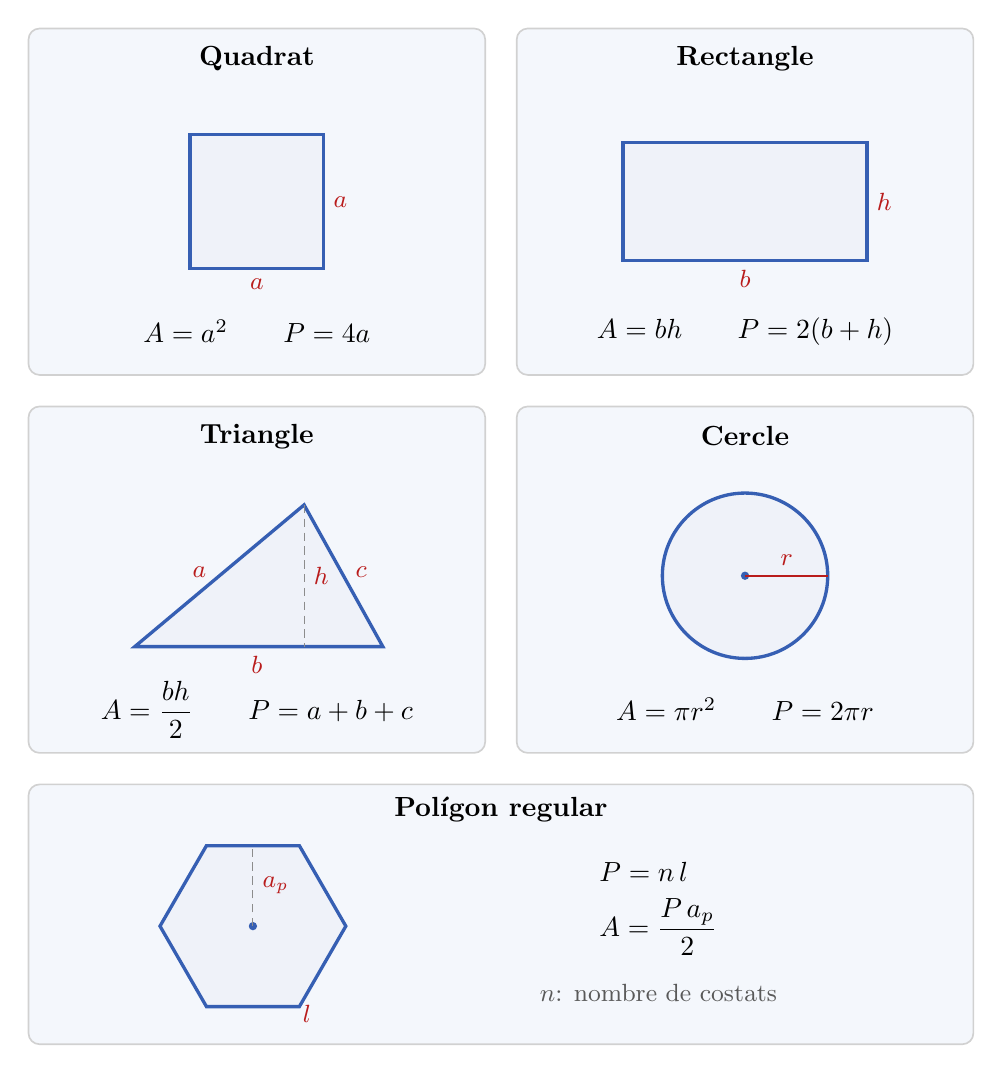
\begin{tikzpicture}[x=1cm,y=1cm]
  \begin{scope}[shift={(0,8.5)}]
    \draw[panell] (0,0) rectangle (5.8,4.4);
    \node[titol] at (2.9,4.02) {Quadrat};
    \draw[figura] (2.05,1.35) rectangle (3.75,3.05);
    \node[etiqueta, below] at (2.9,1.35) {$a$};
    \node[etiqueta, right] at (3.75,2.2) {$a$};
    \node at (2.9,.55) {$A=a^2\qquad P=4a$};
  \end{scope}

  \begin{scope}[shift={(6.2,8.5)}]
    \draw[panell] (0,0) rectangle (5.8,4.4);
    \node[titol] at (2.9,4.02) {Rectangle};
    \draw[figura] (1.35,1.45) rectangle (4.45,2.95);
    \node[etiqueta, below] at (2.9,1.45) {$b$};
    \node[etiqueta, right] at (4.45,2.2) {$h$};
    \node at (2.9,.55) {$A=bh\qquad P=2(b+h)$};
  \end{scope}

  \begin{scope}[shift={(0,3.7)}]
    \draw[panell] (0,0) rectangle (5.8,4.4);
    \node[titol] at (2.9,4.02) {Triangle};
    \coordinate (A) at (1.35,1.35);
    \coordinate (B) at (4.5,1.35);
    \coordinate (C) at (3.5,3.15);
    \draw[figura] (A)--(B)--(C)--cycle;
    \draw[guia] (C)--(3.5,1.35);
    \node[etiqueta, below] at (2.9,1.35) {$b$};
    \node[etiqueta, right] at (3.5,2.25) {$h$};
    \node[etiqueta, left] at (2.38,2.3) {$a$};
    \node[etiqueta, right] at (4.03,2.3) {$c$};
    \node at (2.9,.55) {$A=\dfrac{bh}{2}\qquad P=a+b+c$};
  \end{scope}

  \begin{scope}[shift={(6.2,3.7)}]
    \draw[panell] (0,0) rectangle (5.8,4.4);
    \node[titol] at (2.9,4.02) {Cercle};
    \draw[figura] (2.9,2.25) circle (1.05);
    \fill[corba] (2.9,2.25) circle (1.5pt);
    \draw[mesura, thick] (2.9,2.25)--(3.95,2.25);
    \node[etiqueta, above] at (3.43,2.25) {$r$};
    \node at (2.9,.55) {$A=\pi r^2\qquad P=2\pi r$};
  \end{scope}

  \begin{scope}[shift={(0,0)}]
    \draw[panell] (0,0) rectangle (12,3.3);
    \node[titol] at (6,2.98) {Polígon regular};
    \begin{scope}[shift={(2.85,1.5)}]
      \draw[figura]
        (0:1.18) -- (60:1.18) -- (120:1.18) --
        (180:1.18) -- (240:1.18) -- (300:1.18) -- cycle;
      \fill[corba] (0,0) circle (1.5pt);
      \draw[guia] (0,0)--(90:1.02);
      \node[etiqueta, right] at (90:.52) {$a_p$};
      \node[etiqueta, below right] at (-60:1.02) {$l$};
    \end{scope}
    \node[align=left] at (8.0,1.72)
      {$P=n\,l$\\[5pt]$A=\dfrac{P\,a_p}{2}$};
    \node[font=\small, text=black!65] at (8.0,.65)
      {$n$: nombre de costats};
  \end{scope}
\end{tikzpicture}
\end{document}
